% This file was converted to LaTeX by Writer2LaTeX ver. 1.2
% see http://writer2latex.sourceforge.net for more info
\documentclass[a4paper]{article}
\usepackage[utf8]{inputenc}
\usepackage[T1]{fontenc}
\usepackage[english]{babel}
\usepackage{amsmath}
\usepackage{amssymb,amsfonts,textcomp}
\usepackage{color}
\usepackage[top=2cm,bottom=2cm,left=2cm,right=2cm,nohead,nofoot]{geometry}
\usepackage{array}
\usepackage{hhline}
\usepackage{hyperref}
\hypersetup{pdftex, colorlinks=true, linkcolor=blue, citecolor=blue, filecolor=blue, urlcolor=blue, pdftitle=, pdfauthor=abhinando, pdfsubject=, pdfkeywords=}
\usepackage[pdftex]{graphicx}
% Text styles
\newcommand\textstyleInternetlink[1]{\textcolor{blue}{#1}}
% Footnote rule
\setlength{\skip\footins}{0.119cm}
\renewcommand\footnoterule{\vspace*{-0.018cm}\setlength\leftskip{0pt}\setlength\rightskip{0pt plus 1fil}\noindent\textcolor{black}{\rule{0.25\columnwidth}{0.018cm}}\vspace*{0.101cm}}
\title{}
\author{abhinando}
\date{2012-09-01}
\begin{document}
\clearpage\setcounter{page}{1}{\raggedleft\bfseries
Wolves, Dreams, Transformations
\par}

{\raggedleft\bfseries
Wölfe, Träume, Verwandlungen 
\par}


\bigskip


\bigskip


\bigskip


\bigskip


\bigskip


\bigskip


\bigskip


\bigskip


\bigskip


\bigskip


\bigskip


\bigskip


\bigskip


\bigskip


\bigskip


\bigskip


\bigskip


\bigskip


\bigskip


\bigskip


\bigskip

{\raggedleft
poems by
\par}

{\raggedleft\bfseries
Bhikkhu Abhinando
\par}


\bigskip


\bigskip


\bigskip


\bigskip

{\bfseries
Wolves, Dreams, Transformations}

{\bfseries
Wölfe, Träume, Verwandlungen}


\bigskip


\bigskip


\bigskip

poems


\bigskip


\bigskip

Bhikkhu Abhinando


\bigskip


\bigskip


\bigskip


\bigskip


\bigskip


\bigskip


\bigskip


\bigskip


\bigskip


\bigskip


\bigskip


\bigskip


\bigskip


\bigskip


\bigskip


\bigskip


\bigskip


\bigskip


\bigskip


\bigskip


\bigskip


\bigskip


\bigskip


\bigskip


\bigskip

 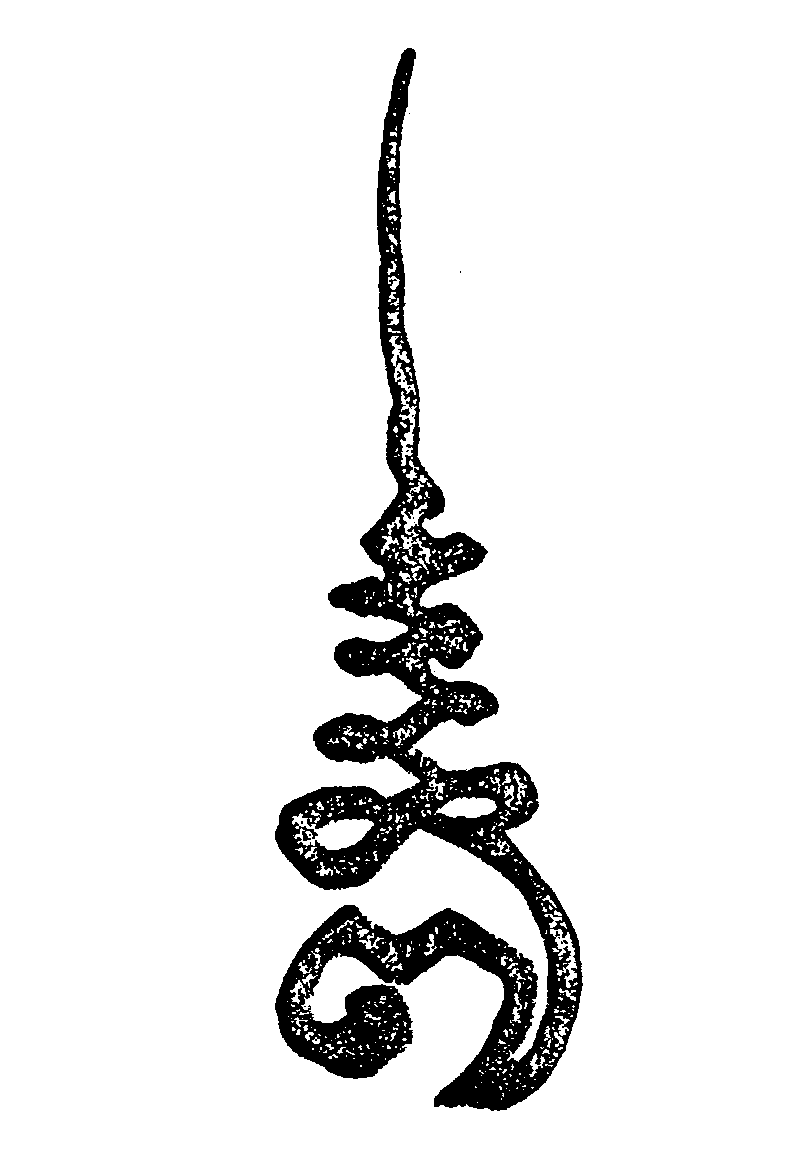
\includegraphics[width=2.432cm,height=3.498cm]{Wolfefinal2-img001.png} 


\bigskip

Aruna Publications

\clearpage
\bigskip


\bigskip

This book has been sponsored for free distribution.


\bigskip


\bigskip

Aruna Ratanagiri: Harnham Buddhist Monastery

2 Harnham Hall Cottages

Harnham, Belsay

Northumberland

NE20 0HF

United Kingdom


\bigskip


\bigskip

{\color{black}
\href{http://www.ratanagiri.org.uk/}{\textstyleInternetlink{www.ratanagiri.org.uk}}}

{\color{black}
\href{http://www.forestsangha.org/}{\textstyleInternetlink{www.forestsangha.org}}}


\bigskip


\bigskip


\bigskip


\bigskip


\bigskip


\bigskip


\bigskip


\bigskip


\bigskip


\bigskip

\textbf{© }2012\textbf{ }Bhikkhu Abhinando 


\bigskip

No part of this book may be reproduced in any form without written permission from the author.


\bigskip

ISBN \textcolor{red}{XXXXXXXXXXXX}


\bigskip

\textit{Animals that Visit Me at Night} first appeared in \textit{Urthona.}


\bigskip


\bigskip


\bigskip

Design and layout: Gambh\=\iro Bhikkhu


\bigskip

Many thanks to Ajahn Sucitto, Linda France and Graham Brown for their help with the translations.


\bigskip


\bigskip

If you would like to contribute to the activities of Aruna Ratanagiri Buddhist Monastery including the publication of
materials for free distribution, please contact the address above or go to http://www.ratanagiri.org.uk/fund.htm


\bigskip


\bigskip

Printed in the U.K. at Remous Ltd

Sherborne, Dorset

\clearpage
\bigskip


\bigskip


\bigskip


\bigskip


\bigskip


\bigskip


\bigskip

{\itshape
Love is most nearly itself}

{\itshape
when here and now cease to matter.}


\bigskip

\ \ \ \ T.S. Eliot, \textit{East Coker}

\clearpage
\bigskip

{\bfseries
I}

\clearpage{\bfseries
Die Fliegen}


\bigskip


\bigskip

Ich fand einen weichen Sitz aus Moos

zwischen den Wurzeln einer Lärche.


\bigskip

Alles ist still, 

außer dem Wind in den Wipfeln,

den Vogelstimmen

und dem Gesumm beharrlicher Fliegen.


\bigskip

Ich trinke grünen Tee 

aus einer Thermosflasche,

blättere in einem Buch

„lebensbejahender“ Gedichte;


\bigskip

mal nehm ich es auf,

mal leg ich es weg:


\bigskip

Vielleicht ist Liebe

allein zu sein

in einem Wald voller Fliegen – 


\bigskip

freigelassen verschwinden

Sehnsucht und Verlangen

in den Farnen und hohen Gräsern

eines grünen Horizontes,


\bigskip

und für den Augenblick bleibt nur

die stille Lyrik dessen, was geschieht

zwischen Ankunft 

und Rückkehr

an den Ort meiner Herkunft.


\bigskip

\clearpage
\bigskip

{\bfseries
The Flies}


\bigskip


\bigskip

I found a soft seat of moss 

between the roots of a larch.


\bigskip

Everything is silent, 

apart from the wind in the trees, 

birdsong

and the buzzing of persistent flies.


\bigskip

Sipping green tea from a thermos 

I leaf through a book 

of ‘life-affirming’ poems, 


\bigskip

picking it up and putting it down:


\bigskip

perhaps love is

to be alone

in a forest full of flies – 


\bigskip

set free, longings and desires

disappear into the ferns and tall grasses

of a green horizon


\bigskip

and for the moment there remains only 

the quiet poetry of what happens

between coming here

and going back where I came from.

\clearpage{\bfseries
Vier Schritte in der Wüste}


\bigskip

{\itshape
\ \ \ \ für Chandra}


\bigskip

Vier Schritte in der Wüste – 

ein schräger Vogel, neuromantisch

tönend in der Nacht. 


\bigskip

Auf der anderen Schale liegt

im Gleichgewicht die Welt.

Sie fühlt genau wies steht

um unsere Wunden.


\bigskip

Vier Schritte in der Wüste $-$

es ist die Sehnsucht die wir wollen,

nicht die Bilder an der Wand

einer ausgemalten Zukunft.


\bigskip

Wäre ich ein Haus,

ich hätte keine Wände;

wäre ich ein Strauch,

nur meine Wurzeln hielten aus;

wäre ich ein Fluss,

auf meinem Grunde rollten die Steine

gegen jegliches Gesetz.


\bigskip

Vier Schritte in der Wüste – 

ein Notturno auf der Suche

nach der verlorenen Richtung:

Der wahre Weg

weicht ab.


\bigskip


\bigskip

\clearpage\subsection[Four Steps in the Desert]{\color{black} Four Steps in the Desert}
\emph{\textup{\textcolor{black}{\ \  \ \ \ \ \ }}}\emph{\textcolor{black}{for Chandra}}


\bigskip

{\color{black}
Four steps in the desert – }

{\color{black}
a strange bird singing}

{\color{black}
neo-romantic hymns to the night.}


\bigskip

{\color{black}
On the other scale the world}

{\color{black}
holds the balance,}

{\color{black}
knowing precisely the weight}

{\color{black}
of our wounds.}


\bigskip

{\color{black}
Four steps in the desert – }

{\color{black}
it is the longing we desire,}

{\color{black}
not the pictures on the wall}

{\color{black}
of an imagined future.}


\bigskip

{\color{black}
If I were a house,}

{\color{black}
I would have no walls;}

{\color{black}
if I were a bush,}

{\color{black}
only my roots would endure;}

{\color{black}
if I were a river,}

{\color{black}
in my depths the stones would roll}

{\color{black}
against any law.}


\bigskip

{\color{black}
Four steps in the desert – }

{\color{black}
a nocturne in search}

{\color{black}
of the lost direction:}

{\color{black}
the true way}

{\color{black}
strays off the path.}


\bigskip

\clearpage{\bfseries
Herzwolf}


\bigskip

Kobaltblaue Augen

brennt eure Schneisen

in die schlaflose Landschaft:


\bigskip

Herzwolf,

zähl meine Schafe!


\bigskip

\clearpage{\bfseries
Heartwolf}


\bigskip

Cobalt-blue eyes 

burn your swathes

into the sleepless landscape:


\bigskip

Heartwolf,

count my sheep!


\bigskip


\bigskip

\clearpage{\bfseries
\textit{Hotel} \textit{Zur Guten Zukunft}}


\bigskip

Im \textit{Hotel} \textit{Zur Guten Zukunft} sind alle Betten

von häuslichen Utopien belegt

Gewissensimplantate wachsen 

wie Pilzbefall an den Wänden

verbreiten Herzmorchelmief


\bigskip

Du fliehst in den ummauerten Garten

Hier singen die Sterne wie Nadelstiche

eine Fischgräte leuchtet 

eine Amsel bleibt stumm

blinzelt dich an

und würgt einen Kirschkern hervor


\bigskip

Ganz woanders zwischen Euphrat und Tigris 

wuchert der Blütenteppich der Leukämie

Verarmtes Uran bettelt in der Wüste~ 

dreiäugige Kinder beißen zurück


\bigskip

Du wanderst im Kreis in deinem Garten

Hier singen die Steine wie glühende Knochen

eine Fischgräte leuchtet

am Deckel der Nacht


\bigskip

\clearpage{\bfseries\itshape
Hotel Good Future}


\bigskip

In the \textit{Hotel Good Future} all rooms

are taken by homely utopias

Implants of conscience grow

like fungal infestations on the walls

spread the stink of mushroom-hearts


\bigskip

You escape into the walled garden

Here the stars sing like pinpricks

a fishbone shines

a blackbird stays silent

blinks at you

and regurgitates a cherry pip


\bigskip

In quite a different place 

between Tigris and Euphrates

sprawls the flower carpet of leukaemia 

Depleted uranium goes begging in the desert

three-eyed children bite back


\bigskip

You walk in circles in your garden

Here the stones sing like luminous bones

a fishbone shines

on the lid of the night


\bigskip

\clearpage{\bfseries
Der Sprachschlucker}


\bigskip

Er gab das Reden niemals gänzlich auf,

doch früh fand er im Schweigen

seine eigentliche Leidenschaft.

Er stand am Rande der Gespräche

und verschluckte was er hörte

$-$ ein diskreter,

bodenloser Schlund.


\bigskip

Die anderen sahen sich oft

verstört nach ihm um,

wenn sie bemerkten, 

dass sie schon vergessen hatten 

wovon sie eben sprachen.


\bigskip

Er aber schwieg, höflich verschlossen

mit seinem wie

mit etwas Entferntem beschäftigten Blick.


\bigskip

\clearpage{\bfseries
The Language-Eater}


\bigskip

He never entirely gave up talking

but early on he found in silence

his real passion.

He stood at the margin of conversations

and swallowed what he heard

$-$ a discreet 

bottomless throat.


\bigskip

Often the others turned towards him 

perplexed

when they noticed

they had already forgotten

what they had just talked about.


\bigskip

But he kept his silence, politely withdrawn

his eyes appearing to be \ occupied 

with something in the distance.

\clearpage
\bigskip

{\bfseries
Sostenuto}


\bigskip

Eine Stimme,

lauschende Stimme,

tastet uns ab;


\bigskip

niemandes Stimme,

herrenloser Hund

auf der Suche nach Heimat;


\bigskip

Kinderstimme,

kleiner Stotterkäfer

auf der Herzwand des Leidens:


\bigskip

des Eichhörnchens 

panische Bahnen

in unserem Wintergarten;


\bigskip

der Heckenbraunelle

lautlose Neugier,

lautlose Flucht.


\bigskip

Wer spricht?


\bigskip

\clearpage{\bfseries
Sostenuto}


\bigskip

A voice, listening 

voice, sensing us

with gentle fingers;


\bigskip

nobody’s voice,

stray dog

seeking a home;


\bigskip

child’s voice,

little stutter-bug,

crawling on the blistered heart:


\bigskip

the squirrel’s 

panicky tracks

through our winter-garden;


\bigskip

the dunnock’s silent

curiosity,

its soundless escape.


\bigskip

Who speaks?


\bigskip

\clearpage{\bfseries
Tiere die Mich Besuchen in der Nacht}


\bigskip

Ich habe lange nicht mehr von Pferden geträumt.


\bigskip

Aber dafür träumte ich von Stachelschweinen.

Die wimmelten furchtlos

wie Stachelratten 

unter dem Teppich.


\bigskip

Und von fröscheverschlingenden Schlangen.

Die hatten auch dich im Visier.

Die Frösche verschwanden lautlos,

beschwerten sich nicht.


\bigskip

Und vom Skorpion.

Schwarz und metallen raschelnd kam er daher,

jede Tür die ich zwischen uns warf,

blieb einen Spalt weit geöffnet.


\bigskip

Und von einem kleinen Bären.

Der war krank, klammerte sich 

kläglich an meinen Hals.

Ob er gesund ward, weiß ich nicht.


\bigskip

Gestern endlich erschienen die Wölfe:


\bigskip

Wir lagerten uns still in die Dämmerung.

Der große schwarze ließ seine Schnauze

auf meiner Schulter ruhn, sah mich an.

So, gemeinsam, waren wir sicher für die Nacht.


\bigskip

\clearpage{\bfseries
Animals That Visit Me at Night}


\bigskip

It’s a long time since I dreamt of horses. 


\bigskip

I dreamt of porcupines instead.

They were teeming fearlessly

like spiked rats

under the carpet.


\bigskip

And of frog-swallowing snakes.

They had an eye on you as well.

The frogs, in between the deadly fangs,

did not complain. 


\bigskip

And of a scorpion.

It came black and rustling with a metal sound.

Every door I slammed between us

remained open just a gap.


\bigskip

And then there was the little bear.

It was sick, clinging 

pathetically to my neck.

Whether it recovered, I do not know.


\bigskip

Finally, yesterday, the wolves arrived.


\bigskip

At dusk they settled quietly around me.

The big black one rested its muzzle

on my shoulder and looked at me.

So, together, we were safe for the night.


\bigskip

\clearpage{\bfseries
Schattenwolf}


\bigskip

{\itshape
Solo la nieve sabe}

{\itshape
la grandeza del lobo.}

\textit{\ \  \ \ \ \ \ \ }Leopoldo María Panero


\bigskip

Nur der Schnee weiß

von der Größe des Wolfes

der unsere Schatten verschlingt


\bigskip

Nur die Leere unter dem Mond

versteht seine Sprache

die versöhnt wie lebendiges Wasser


\bigskip

Nur die Krüppelkiefer 

und der Felsen auf dem er liegt

wachen über seinen Schlaf


\bigskip

während der Schmerz schreit

und das Sonnenlicht

seine Spuren verwischt


\bigskip

\clearpage{\bfseries
Shadow-Wolf}


\bigskip

{\itshape
Solo la nieve sabe}

{\itshape
la grandeza del lobo.}

\textit{\ \ \ \ \ \ \ \ \ \ }Leopoldo María Panero


\bigskip

Only the snow knows

the greatness of the wolf

that swallows our shadows


\bigskip

Only the void beneath the moon

understands his language

that reconciles like living water


\bigskip

Only the twisted pine

and the rock on which he lies

watch over his sleep


\bigskip

while the pain screams

and sunlight

wipes out the tracks


\bigskip


\bigskip

\clearpage{\bfseries
Kein Ende in Sicht}


\bigskip

Am Ende sitz ich allein auf dem Berg,

in einem Haufen Schnee.

Entweder ich erfriere, oder

der Allmächtige

holt mich ab.


\bigskip

*****


\bigskip

Als lebender Fleischkloß lieg ich auf dem Fließband,

wie eine Wurst gewickelt in meine rosa Haut;

ein weit geöffneter Schlund und ein einziges, flehendes Auge:

{\itshape
Doktor, Doktor, sagen sie mir, dass ich noch zu retten bin.}

Der aber zuckt mit den Achseln, drückt einen Knopf –

das Fließband rasselt weiter.


\bigskip

*****


\bigskip

Meine Schwestern und Brüder stochern ratlos 

in den Trümmern des eingestürzten Tempels.

Ich wende mich ab, geh fort, 

rutsche die Gasleitung entlang

über den Fluss, in Gegenrichtung zum Verkehr

auf der einzigen Brücke.


\bigskip

Auf halbem Weg über den Fluss lass ich mich fallen und lande

auf einem Ausflugsdampfer,

besorgt, dass ich keinen Fahrschein habe.

Die Freunde lachen – 

sie haben für mich bezahlt.


\bigskip

*****


\bigskip


\bigskip

Die Reise endet in einer indischen Stadt;

wir legen am Marktplatz an, ich bestaune

die Gruppe der Fakire auf ihren Nagelbetten.

Dann verliere ich mich im bunten Gemenge,

kann mich nirgendwo mehr sehen.


\bigskip

*****


\bigskip

Wir sitzen im Straßencafé,

du trinkst dein Bier, ich meinen Tee.

Du erzählst mir vom Leid deines Lebens,

ich höre zu, ein Seufzer

jede Naht meines Wesens.


\bigskip

*****


\bigskip

Du erschlägst den Fremden aus Eis, 

der meine Hand in seinem Schraubstock hält.

Sobald die Axt in seinen Schädel dringt,

schmilzt er und sickert in den Teppich:

Unsere Freundschaft ist gerettet.


\bigskip

*****


\bigskip

Ich führe meine Krieger auf das Blaue Plateau.

Hier kann der Feind uns nicht erschießen;

er steht gelähmt in seiner blauen Uniform, 

denn hier, auf dem heiligen Berg, sind wir eins.


\bigskip


\bigskip

\clearpage
\bigskip

{\bfseries
No End in Sight}


\bigskip


\bigskip

In the end I sit alone on the summit

in a heap of snow.

Either I freeze to death

or the Almighty

picks me up.


\bigskip


\bigskip

****


\bigskip

A living lump of meat, I lie on the conveyor belt,

wrapped in my pink skin like a sausage;

one gaping throat and one eye begging:

{\itshape
Doctor, doctor, please tell me I'll be okay.}

He shrugs his shoulders, presses a button – 

the belt rattles on.


\bigskip


\bigskip

*****


\bigskip

My sisters and brothers poke helplessly

through the debris of the wrecked temple.

I turn around, go away, 

crawling along the gas pipe 

crossing the river against 

the one-way traffic on the only bridge.


\bigskip

Half-way across the river I let go

and land on a steam boat

worried that I haven't got a valid ticket.

My friends laugh:

they have paid for me.


\bigskip


\bigskip

*****


\bigskip

Our journey ends in an Indian city.

Our boat moors at the market place.

I marvel at the group of fakirs on their nail beds.

Then I get lost in the colourful crowd,

can't see myself anywhere anymore.


\bigskip


\bigskip

***


\bigskip

We sit in the street-café.

You drink your beer, I drink my tea.

You tell me about the pain of your life.

I listen, every seam 

of my being a sigh.


\bigskip


\bigskip

***

You destroy the frozen stranger,

who holds my hand in his vice.

As soon as the axe enters his head,

he melts and seeps into the carpet.

Our friendship is saved.


\bigskip

{\itshape
******}


\bigskip


\bigskip

I lead my warriors up to the Blue Plateau.

Here the enemies can’t shoot us;

they are paralysed, because up here, 

on the holy mountain, we are one.


\bigskip


\bigskip

\clearpage{\bfseries\itshape
Engel Hab Ich Mir Abgewöhnt }


\bigskip

Der Engel mit dem Nesselflügel streift mein Gesicht,

heute, gestern, immer wieder,

und von meinen vertrocknenden Lippen

starten die Vögel.


\bigskip

Der Engel mit dem Kirschblütenlächeln

vergibt mir schon wieder ein von der Zeit 

längst überholtes Versprechen.

Sein hilfloser Blick 

durchlöchert mich.


\bigskip

Der Engel mit den verschrumpelten Händen

stellt Fallen auf – ich weiß nicht wofür,

ist er doch selbst wie ein Nagetier

in den Kellergängen 

des guten Gewissens.


\bigskip

Der Engel der Verwesung – 

Schutzheiliger der Verschwundenen –

brach sich einmal an mir seine Flügel

wie ein Vogel, ein ganz gewöhnlicher.


\bigskip

Jetzt wetzt er seinen Schnabel

an meinen steinharten Lippen.


\bigskip

Ich bin allein mit meinem Verdacht

und den scheppernden Sternen

einer mechanischen Nacht, 

wie ein unvollendeter Engel,

der wartet

auf sein Federkleid. 

\clearpage{\bfseries\itshape
I Abandoned the Habit of Angels }


\bigskip

The angel with the nettle-wing touches my face,

today, yesterday, and again and again,

and the birds take off

from my withering lips.


\bigskip

The angel with a smile of cherry-blossom

forgives me yet another promise

outlived by time.

His helpless gaze

rips me to pieces.


\bigskip

The angel with shrivelled hands

puts out traps – I don't know for what 

as he himself is a rodent

in the catacombs

of innocence.


\bigskip

The angel of putrefaction – 

patron saint of the disappeared – 

once broke his wings on me,

like an ordinary bird.


\bigskip

Now he sharpens his beak

on my stony lips.


\bigskip

I am alone with my suspicion

and the clanking stars

of a mechanical night

like an unfinished angel 

waiting for his plumage.


\bigskip

{\bfseries
Einsiedler auf Düsterem Berg}


\bigskip


\bigskip

der Körper voll bellender Hunde

der Geist voll fehlender Esel


\bigskip

das Herz eine Landschaft von Farbe erobert

ein Ofen der Unruhe brennt

Steine zu Atem verwandelt 


\bigskip

das Ende jeder Fantasie

ein Finger der auf ein Opfer zeigt


\bigskip

Sehnsüchte und Verlangen

ein einziger Geschmack für tausend Fliegen

und niemand den man nach Gründen 

fragen kann


\bigskip

während der Atem zur Wolke wird

die den Regen bringt

den das Land begehrt 

\clearpage
\bigskip

{\bfseries
Hermit on Sullen Mountain}


\bigskip


\bigskip

the body full of barking dogs

the mind of missing donkeys


\bigskip

the heart a landscape conquered by colour

an oven fuelled by restlessness

turning stones to breath


\bigskip

the end of every fantasy

a finger pointing to a victim


\bigskip

aspirations and desires

one taste to a million flies

and no one to ask for reasons


\bigskip

while the breath turns to cloud

carries the rain the land is praying for

\clearpage{\bfseries
Schwester}


\bigskip

\textit{Sie raucht, hat grüne Augen, kommt vom Meer} $-$

und verlor ihren Weg 

im eigenen Herzen.


\bigskip

In einem brennenden Kleid,

mit einem Lächeln, das nicht zu löschen versucht,

mit Füßen aus Schnee, 


\bigskip

tappt sie durch diesen 

$-$ fast meinen $-$

eingeschlossenen Himmel,


\bigskip

{\itshape
ein Auge, das eine Sonne sieht,}

\textit{eine Hand, die eine Erde fühlt},

ein Verstand, der eine Lüge riecht


\bigskip

und vergibt.

Wenn ich jetzt die Begegnung wähle,

mit dem Finger des Zweifels


\bigskip

an der Wunde rühre,

uns vorlese 

aus der offengelegten Schrift,


\bigskip

könnten wir gemeinsam brennen, vielleicht,

bis eines Tages nur der Himmel

übrigbleibt.


\bigskip

\clearpage{\bfseries
Sister}


\bigskip

{\itshape
She smokes, has green eyes, comes from the sea $-$}

and has lost her way

inside her heart.


\bigskip

In a burning dress, with a smile 

not trying to put out the flames,

with feet of snow


\bigskip

she gropes through this

$-$ almost mine $-$

enclosed sky,


\bigskip

{\itshape
an eye that sees a sun,}

\textit{a hand that feels an earth}.

A mind that smells a lie


\bigskip

and forgives.

If now I choose to meet her,

to put the finger of doubt


\bigskip

softly on the wound

and read for us

from the uncovered script,


\bigskip

we could burn together, perhaps,

until one day only the sky 

is left.


\bigskip


\bigskip


\bigskip

\clearpage{\bfseries
Die Stille in Mailand}

\ \ \ \ \textit{für Chandra}


\bigskip

Stille der Großstadt,

ungelenke Eroberin,

sanfter Clown, Alltagsclown, 

der horcht und der hört.


\bigskip

Stille mit den weit geöffneten Augen,

staunende Stille,

die uns an ihren warmen

Händen führt $-$


\bigskip

an den Stadtrand, wo

die Straßen sich verlaufen,

wo sie enden, in Halden

und Abstellplätzen,


\bigskip

an einer stehengelassenen 

Mauer, oder

in einem stummen Feld.

Mosaik der Stille, 


\bigskip

zusammengesetzt

aus weggeworfenen

Requisiten des Alltags,

aus Gesten und Blicken 


\bigskip

die vorübergingen

im Zentrum der Stadt; 

wo was wir tun,

was wir nehmen


\bigskip

oder liegenlassen,

zum stillen Kunstwerk deiner Sprache wird.

Plötzlich bleibst du stehen

und siehst mich an:


\bigskip

stille Rose am Mantelkragen,

Schneefall und aufgelesener Schirm.

Die Angst frisst dir aus den Händen,

deine Stimme ist firm.


\bigskip

\clearpage{\bfseries
Silence in Milan}

{\itshape
\ \ for Chandra}


\bigskip

Silence of the big city,

clumsy conqueress,

gentle clown, everyday-clown,

that listens and hears.


\bigskip

Silence with wide open eyes,

marvelling silence

that leads us

with warm hands $-$


\bigskip

to the outskirts where

the streets lose themselves,

where they end in skips

and parking bays, 


\bigskip

at left-behind walls

or in mute fields.

Mosaic of silence, 

put together


\bigskip

from thrown-away requisites 

of daily life, 

from gestures and glances of those

who passed us


\bigskip

in the city-centre, 

where everything we do,

everything we pick up 

or leave behind


\bigskip

becomes the silent art

of your language. 

Suddenly you stop 

and look at me:


\bigskip

silent rose on the lapel of your coat,

snowfall and umbrella somewhere found.

Fear eats out of your hand,

your voice holding its ground.

\clearpage
\bigskip


\bigskip

{\bfseries
An der Tür}


\bigskip

Zweifelmus

von Dogmen umschnüffelt

Die Liebe ist anders. Dein

{\itshape
ich weiß nicht}

zerrt an der Tür

\clearpage{\bfseries
At the Door}


\bigskip

A mush of doubt

with sniffing dogmas all around it

Love is different. Your

{\itshape
don't know}

pulls at the door

\clearpage{\bfseries
II}


\bigskip

\clearpage{\bfseries
Traumkasten}


\bigskip

heraus springt

der ritter aus titanium

auf seinem silbernen pferd


\bigskip

und erobert was zu erobern ist


\bigskip

zurück bleibt

die wilde heilige

tanzend um sich schlagend


\bigskip

als wüsste sie was niemand weiß


\bigskip

herum steht

das schwarze fohlen

das zärtlich an den schultern


\bigskip

meiner freunde knabbert


\bigskip


\bigskip

\clearpage{\bfseries
Dreambox}


\bigskip

out jumps

the titanium knight

on his silver horse


\bigskip

and conquers what is to be conquered


\bigskip

inside remains

the wild woman saint

dancing and hitting out 


\bigskip

as if she knew what no one knows


\bigskip

there lingers

the black colt

carefully nibbling 


\bigskip

the shoulders of my friends


\bigskip

\clearpage{\bfseries
Hohes Gras und Meer }


\bigskip

Eine Landschaft mit Lagerhäusern:

hohes Gras, rostendes Gerät,

wehendes Papier.


\bigskip

Hier unterliegen wir dem Regen

und dem beinahe zärtlichen

Anruf der Möwen.


\bigskip

{\itshape
Steigende Flut}

{\itshape
in meinem Traum;}

{\itshape
die Nachbarin empfiehlt }

{\itshape
den Tauchanzug.}

{\itshape
Zögernd schau ich }

{\itshape
auf haushohe Wellen.}


\bigskip

Ich erinnere einen Tag mit hohem Fieber, 

allein

in der Wohnung einer Bekannten,


\bigskip

mit einem nie zu Ende

gelesenen Buch der Anaïs Nin,

in Sichtweite dieser Landschaft.


\bigskip

{\itshape
Was siehst du im Fenster?}

{\itshape
Wo ist das Meer?}

{\itshape
Standen wir nicht in der Mündung des Flusses?}

{\itshape
Und plötzlich kamen von zwei}

{\itshape
Seiten die Wellen,}

{\itshape
die Küste schwamm uns davon.}


\bigskip

Unter Kolumbiens sengender Sonne

half ich einmal den Fischern am Strand

beim Einholen der Netze,


\bigskip

sah zwei flüchtende Männer,

wechselte ein Wort mit ihren 

bewaffneten Verfolgern,


\bigskip

las im schmalen Schatten der Böschung

Heine, Rimbaud

und Baudelaire.


\bigskip

{\itshape
Ich verlasse die Stadt.}

{\itshape
Bald erreicht mich }

{\itshape
der Flüchtlingsstrom}

{\itshape
in zerknitterter Landschaft:}

{\itshape
Wassermassen nahen }

{\itshape
von überall her.}


\bigskip

Ich erinnere die Blicke der schönen Frauen von Riohacha,

den Haifischkopf

und das undurchsichtige Meer.

~

\clearpage{\bfseries
High Grass and the Sea}


\bigskip

A landscape with warehouses:

high grass, rusting equipment,

drifting paper.


\bigskip

Here we succumb to the rain 

and the almost affectionate 

call of the gulls.


\bigskip

{\itshape
Rising flood}

{\itshape
in my dream;}

{\itshape
the neighbour recommends}

{\itshape
a diving-suit.}

{\itshape
Hesitating, I stare}

{\itshape
at the enormous waves.}


\bigskip

I remember a day with high fever,

alone

in the flat of a friend,


\bigskip

with a never finished

novel by Anaïs Nin,

within sight of this landscape.


\bigskip

{\itshape
What do you see in the window?}

{\itshape
Where is the ocean?}

{\itshape
Didn’t we stand in the river-mouth?}

{\itshape
And suddenly the waves came}

{\itshape
from two directions,}

{\itshape
the coast swimming away from us.}


\bigskip

Beneath the torrid sun of Columbia

I once helped the fishermen on the beach 

hauling in their nets,


\bigskip

saw two fleeing men, chatted

with their armed pursuers,


\bigskip

read in the thin shade of the embankment

Heine, Rimbaud

and Baudelaire.


\bigskip

{\itshape
I leave the city.}

{\itshape
Soon the stream of refugees}

{\itshape
catches up with me}

{\itshape
in a crumpled landscape:}

{\itshape
masses of water closing in}

{\itshape
from everywhere.}


\bigskip

I remember the gaze of the beautiful women from Riohacha,

the shark’s head

and the inscrutable sea.


\bigskip

\clearpage{\bfseries
Aquamarina}


\bigskip

Ich schau in mich hinein

wie in ein Aquarium:

Anemonen, Wasserfarn, blaugrün

leuchtende Algen $-$

im Zentrum ein magnetisches 

Schwarz: die Pupille.


\bigskip

Auf ihrem Grund

wandelt das Beziehungswesen,

Seeigelanemonenschwamm $-$

weichgefüllt mit festem Kern:

in alle Richtungen fühlen

die robust-sensiblen Flimmerfinger.


\bigskip

Bevor das Wasser mich übernahm,

saß mein schwarzes Skelett

als riesiges Insekt

auf dem Fels $-$ 

eine Feder,

gespannt vor dem Sprung.


\bigskip

Nun tauche ich auf

mit Dreizack und Krone,

gutmütigem Blick,

schwabbelig in meiner Gummihaut,

allein im Meer: nur mir

hat man es anvertraut.


\bigskip


\bigskip

\clearpage{\bfseries
Aquamarina}


\bigskip

I look into myself,

as if into an aquarium:

anemones, waterfern, algae,

blue green and luminous $-$

and in the centre, magnetically

black: the pupil.


\bigskip

On its bottom 

wanders the relationthing,

seaurchinspongeanemone $-$

with soft innards and a tough core:

its robustly sensitive jitterfingers

feel into all directions.


\bigskip

Before the water took me over,

my black skeleton sat

like a huge insect

on the stool $-$

a taut spring,

ready to jump.


\bigskip

Now I surface,

with trident and crown,

good-natured gaze,

flabby under my rubbery skin,

alone in the sea: to me alone

it was entrusted.


\bigskip


\bigskip

\clearpage{\bfseries
Auf dem Weg nach Yucatán }

{\itshape
für Daina }


\bigskip

{\bfseries\itshape
I. Die Nacht}


\bigskip

Mit gesenkten Augenlidern 

sah ich die Leere vor

und nach den Visionen: ich war

die Erde unter dem Schlachtfeld,

dankbar für das Werk der Insekten.


\bigskip

Ich höre die Stille vor

und nach dem Versprechen: ich breite

mich aus wie die Spur eines Lächelns,

das immer wieder aufbricht zur Wunde,

sich an dem Tröpfchen Wahrheit zu betrinken.


\bigskip

Meine Gedanken werden seitwärts fliegen, 

heimatlose Raben,

auch wenn es nur Krähen sind,

und mit übertriebener Bescheidenheit

wird meine Geste versuchen

zu erklären:

vor und hinter, über und unter

dem Mond bin ich

die Nacht.


\bigskip

{\bfseries\itshape
II. Der Himmelsläufer}


\bigskip

{\itshape
\ \ der Himmel fällt mir aus den Händen...}

{\itshape
\ \ Ich bin nicht der ich bin}

\textit{\ \  \ \ \ \ \ \ \ \ \ \ \ \ }Leopoldo María Panero


\bigskip

{\itshape
Aber da ist noch eine andere Sonne,}

{\itshape
hinter dem zweiten Horizont,}

{\itshape
dem Ufer überfließenden Reichtums, }

{\itshape
wo die Zukunft den Himmel bewandert}

{\itshape
und nichts die fruchtbare Nacht }

{\itshape
je wirklich verlässt;}

{\itshape
langes Ufer der Nacht, }

{\itshape
wo die ruhiggestellten Visionen des Dichters }

{\itshape
auf eine Nachricht von Lou, }

\textit{auf das Stichwort „Frida“},

{\itshape
erwachen zu einem Lächeln,}

{\itshape
ausuferndem Lächeln,}

{\itshape
in seinem entstellten Gesicht;}

{\itshape
und seine trauergesättigten Augen}

{\itshape
schenken uns ihr wärmendes Licht, }

\textit{und er tanzt, das }Bildnis des Künstlers

als Verwandelter Frosch 

{\itshape
in seinen erhobenen Händen;}

{\itshape
und all die andern Verrückten}

{\itshape
in ihrer unsichtbaren Verkleidung,}

{\itshape
Faune und Feen und Nymphen,}

{\itshape
ein Sommernachtstraum am hellichten Tage,}

{\itshape
taumelnd im Reigen;}

{\itshape
und die reifen Birnen und}

{\itshape
hunderttausend wilde Rosen,}

{\itshape
und der See so warm um unsere Füße,}

{\itshape
der See, mein Herz, der dreizehnte Mond, }

{\itshape
umgekrempelte Sonne,}

{\itshape
funkelnder Bote, ewiger Tag zu deiner}

{\itshape
verführerisch stillen, selbst-}

{\itshape
sicheren Nacht; auch in deinen}

{\itshape
Augen kann ich es sehen,}

{\itshape
und der Himmelsläufer}

{\itshape
hält es wach.}


\bigskip

{\bfseries\itshape
III. Was Wir Seele Nennen}


\bigskip

Und haben wir nicht alle

eine andere Seite?


\bigskip

Plötzlich fällt es mir wieder ein:

die Seele,

oder was wir so nennen,

redet nicht,

sie horcht.


\bigskip

Wenn das Narrenschiff zum zweiten Mal erscheint,

gehen die Mutigen an Bord. 

und ich? $-$


\bigskip

zeichne mit den Zehen im Sand,

sammle die Knochen toter Vögel,

zeige den Sternen 

ihre Artgenossen im Meer,


\bigskip

und denke an die Dichterin:

{\itshape
Was wäre die Liebe, wenn nicht das}

\textit{was aus allen Nähten platzt}.


\bigskip

Zu brennen,

wie die Kerze

sich in Wärme verwandelt und Licht...


\bigskip


\bigskip

\clearpage{\bfseries
Towards Yucatán}

{\itshape
for Daina}


\bigskip

{\bfseries\itshape
I. The Night}


\bigskip

With closed eyelids I saw

the void before

and after the visions: I was

the earth beneath the battlefield,

thankful to the insects for their work.


\bigskip

I hear the silence before

and after the promise: I gain 

ground like the track of a smile

that departs again and again for the wound

to get drunk on a droplet of truth.


\bigskip

My thoughts will fly sideways, 

like homeless ravens,

even if they are just rooks,

and with exaggerated modesty

my gesture will try to explain

that in front, behind, above and below

the moon I am

the night.


\bigskip


\bigskip

{\bfseries\itshape
II. Skywalker}


\bigskip

{\itshape
the sky falls from my hands…}

{\itshape
I am not who I am}

\ \ \ \  Leopoldo María Panero


\bigskip


\bigskip

{\itshape
But there is also another sun,}

{\itshape
behind the second horizon,}

{\itshape
the shore of overflowing abundance, }

{\itshape
where the future walks in the sky}

{\itshape
and nothing really ever}

{\itshape
leaves the fertile night;}

{\itshape
long shore of the night,}

{\itshape
where the poet’s sedated visions }

{\itshape
rise to a message from Lou,}

\textit{to the code word }Frieda, 

{\itshape
to form a single smile,}

{\itshape
escalating smile,}

{\itshape
on his disfigured face;}

{\itshape
and his eyes, saturated with grief,}

{\itshape
bestow us their warming light,}

\textit{and he dances, the }Portrait of the Artist

as a Transformed Frog

{\itshape
held high above his head;}

{\itshape
and all the other lunatics}

{\itshape
in their invisible disguises,}

{\itshape
fauns and fairies and nymphs,}

\textit{a }Summer Night’s Dream \textit{in plain}

{\itshape
daylight, a tumultuous circle dance;}

{\itshape
and the ripened pears and}

{\itshape
a hundred thousand wild roses;}

{\itshape
and the lake so warm around our feet,}

{\itshape
the lake, my heart, the thirteenth moon, }

{\itshape
the sun, turned inside out,}

{\itshape
scintillating walker in the sky, }

{\itshape
eternal day to your seductively quiet,}

{\itshape
self-assured night; }

{\itshape
in your eyes too}

{\itshape
I can see it, and the skywalker}

{\itshape
keeps it awake.}


\bigskip

{\bfseries\itshape
III. What We Call a Soul}


\bigskip

And don’t we all have

another side?


\bigskip

Suddenly I remember:

the soul, or

what we call a soul,

never speaks,

it listens.


\bigskip

When the ship of fools appears a second time

the brave ones board it.

And me? 


\bigskip

I draw with my toes in the sand,

collect bones of dead birds,

show the starfish to their brothers

in the sky,


\bigskip

and think of the poetess:

{\itshape
What else could love be,}

{\itshape
if not what bursts at the seams.}


\bigskip

To burn

like a candle transforms itself

into warmth and light…


\bigskip


\bigskip

\clearpage{\bfseries
Selbstbildnis in Schwarzweiß }


\bigskip


\bigskip

Die Dinge über die ich nicht spreche, 

ziehen die Fäden meiner Träume

und spielen selbst die Nebenrollen,

die der Handlung die Atmosphäre

eines Thrillers verleihen;

sie knabbern wie glühende Würmchen 

an meinen Nerven

und nähren meinen Boden mit Fragmenten

des halbverdauten Verlangens nach Sinn.


\bigskip

Die Dinge die ich verschweige

spitzen die Ohren wie junge Wölfe,

die zum ersten Mal 

das Röhren eines Hirsches hören;

sie winken so wie Unbekannte

auf dem Bahnsteig, auf der Straße, 

mit verlegenem Lächeln;

sie tanzen nachts – die berühmten Gespenster –

auf dem Friedhof meiner Eitelkeit;

sie belauschen mich gern.


\bigskip

Alles was ich nicht sage

manipuliert mindestens einen

meiner zweihundert Schatten;

es wächst in dem verwilderten Garten,

den ich nur besuche, wenn ich zu mehr 

als zwei Dritteln melancholisch bin;

es baut an einem Haus für meine Wölfe \ 

und fuchtelt mit riesigen Spiegeln

ohne mich zu sehen.


\bigskip


\bigskip


\bigskip


\bigskip


\bigskip


\bigskip


\bigskip


\bigskip


\bigskip


\bigskip


\bigskip

{\bfseries
Self-Portrait in Black \& White}

~

The things I do not talk about

move the puppets in my dreams

and play the minor parts that give the plot 

the taste of a thriller;

they nibble like glowing worms

on my nerves,

and nurture my soil with fragments

of the half-digested desire for meaning.

~

The things I keep silent about

prick their ears like young wolves

when they hear a stag’s bell

for the first time;

they wave like strangers

on the platform, in the street,

with embarrassed smiles;

they dance at night – the famous ghosts – 

in the cemetery of my pride;

they love to spy on me.

~

All the things I do not say,

manipulate at least one

of my two hundred shadows;

they grow in the abandoned garden

that I only visit when I am more

than two thirds melancholic;

they are building a house for my wolves 

and wave about with giant mirrors

ignoring my presence.

~

\clearpage{\bfseries
Kaktus in Dünner Luft}


\bigskip


\bigskip

Der Horizont wiegt auf der Höhe seines Herzens,

drückt sanft mit blauen Noten 

auf die Stimmungslage; seine Haut 

wittert in kühlen, leichten,

locker gestaffelten Nebeln

wärmeres Licht. 


\bigskip

In der einfühlsamen Luft \ \ 

zittern seine Blüten: 

Fahnen der Sympathie.

Fast hebt er ab, seinen Bauch

drängt es zur Wolkendecke,

stacheliger Zeppelin.


\bigskip

Er wiegt sich in den wechselnden Winden, 

genießt die Aussicht

und das Ziehen der Leine 

seiner luftigen Wurzel, der Nabelschnur.

Nährstoff steigt ihm durch das Geflecht 

der Kapillaren zu Kopf.


\bigskip

Ein kleiner, horizontale Schmerz in der Brust

hält ihn in schwebender Waage;

er trinkt und atmet und fühlt, 

dass er die ganze winzige Welt 

umarmen kann

mit seinen kitzligen Stacheln.

\clearpage{\bfseries
Cactus in Thin Air}


\bigskip

The horizon weighs in on the level of his heart,

pressing gently with blue notes

on the general mood;

in cool, light, loosely layered mist

his skin senses

warmer light.


\bigskip

His flowers tremble

in empathetic air: 

flags of sympathy.

He almost takes off, belly straining

for the clouds,

spiky zeppelin.


\bigskip

He sways in the changing winds,

enjoys the view

and the pull of the line,

the air root, his umbilical cord. 

Nutriment rises through the web of capillaries

to his head.


\bigskip

A small horizontal pain in his chest

keeps him in fine-tuned suspension,

He drinks and breathes and feels

how he can embrace the entire 

tiny world

with his ticklish spikes.


\bigskip

\clearpage{\bfseries
Wo die Irren Ihn Küssen}


\bigskip


\bigskip

in der von antiken Helden durchzogenen Wüste seines Geistes


\bigskip

auf den vom Schlamm bedrohten Wegen seiner Wünsche


\bigskip

in seinen Wäldern, angefressen von körperlosen Schreien


\bigskip

unter dem krachenden Eis der Seen und Gletscher seines Erbguts


\bigskip

(der wilde Mann mit der Axt

wartet auf wärmeres Wetter)


\bigskip

auf den von unbemannten Schiffen heimgesuchten Meeren seiner Kraft


\bigskip

im Kaufhaus ohne Kassen, ohne Ausgang


\bigskip

(wo er vergessen hat was er sucht)


\bigskip

in den untertunnelten Böden seiner Kindheit


\bigskip

in den von warmen Winden durchwehten menschenleeren Zimmern 


\bigskip

ist er der gejagte Verbrecher sowohl

als auch der Kommissar


\bigskip

werden die Träume von Mal zu Mal komplexer

zunehmend rekursiv


\bigskip

(die Züge kommen niemals an

die Fahrkarten sind nicht gültig

und die Schaffner geben keine Auskunft)


\bigskip


\bigskip


\bigskip

am Ende ist er selbst die Nacht

die ihn aus allen Augen ansieht


\bigskip

jedes moralische Gerüst

in das er seine Zweifel hängt

bricht zusammen unter dem Gewicht


\bigskip

ihm bleibt das Herzgambit

die permanente Öffnung

die Anerkennung

des Anderen

die Versöhnung

mit sich selbst

und Nachsicht


\bigskip

ein Frieden, weder innerlich 

noch äußerlich

aber frei und sehr beweglich

sich ernährend von Verzicht


\bigskip


\bigskip


\bigskip

und so tritt er die blecherne Kanne vor sich her

die Geleise entlang unter blitzendem Himmel

auf dem Weg zur Baracke


\bigskip

wo die Irren ihn küssen

in Missachtung jeglicher Regel des Anstands


\bigskip

\clearpage
\bigskip

{\bfseries
Where He Is Kissed by Lunatics}


\bigskip


\bigskip

in the desert of his mind travelled by classical heroes


\bigskip

on the paths of his desires threatened by mudslides


\bigskip

in his forests half-eaten by disembodied cries


\bigskip

under the thundering ice of the lakes and glaciers of his gene pool


\bigskip

\ \  (the wild man with the axe

\ \  is waiting for warmer weather)


\bigskip

on the ocean of his strength haunted by unmanned ships


\bigskip

in the department store without cash points or exits


\bigskip

\ \  (where he can’t remember what he is looking for)


\bigskip

inside the tunnels that riddle the ground of his childhood 


\bigskip

in the deserted rooms swept by warm winds


\bigskip

he is the villain as well

as the chief inspector


\bigskip

his dreams become more and more complex

increasingly recursive


\bigskip

\ \ (the trains never arrive

\ \ the tickets are not valid

\ \  and the conductors tell him nothing)


\bigskip


\bigskip


\bigskip

in the end he himself is the night

that looks at him

out of every pair of eyes


\bigskip

and every moral scaffolding

onto which he hangs his doubts

collapses under the weight


\bigskip


\bigskip

he is left with nothing but the heart gambit


\bigskip

the constant opening

the recognition

of the other

the reconciliation

with himself

and tolerance


\bigskip

a peace neither inward nor external

but free and flexible

feeding on letting be


\bigskip


\bigskip


\bigskip

and so he kicks the tin can

in front of himself

along the railway tracks

under a lightning sky

on his way to the shed


\bigskip

where the lunatics kiss him

disregarding every rule of good manners


\bigskip

\clearpage{\bfseries
Aureola}


\bigskip

Die quadratischen Augen der Stadt hast du lange verlassen;

das Gängelband besitzergreifender Liebe riss bei deinem ersten Schritt;

dein Pferd brach zusammen in deinen Armen,

weniger kräftig als du gedacht;

die Gitarren sind in den Lagerfeuern verbrannt;

deine wandernden Freunde hatten andere Pläne;

und dein Gebet auf dem hohen Gipfel,

barfuß im Schnee,

brachte keinen Gott um seinen Verstand.


\bigskip

Also die Wüste: du sonnst deine Stacheln;

meist freundlich und scheinbar äußerst genügsam

stehst du still,

treibst deine endlosen, luftigen Wurzeln

in den lockeren Sand

und singst,

webst eine Stimme aus grünem Achat in die Kantate von Düne und Fels,

und dein Wachstum spiegelt sich in den Augen

reglos lauschender Echsen.


\bigskip

\clearpage{\bfseries
Aureola}


\bigskip

The square eyes of the city you have long left behind;

the leash of possessive love snapped with your first step;

your horse collapsed in your arms,

not as powerful as you thought;

the guitars got burned in the bonfires;

your wandering friends had other plans;

and your prayer on the high peak,

barefoot in the snow,

robbed no god of his mind.


\bigskip

So it’s the desert: you are sunning your thorns;

mostly friendly and seemingly easy to please,

you remain still at the centre, 

driving your endless, hollow roots

into the loose sand,

and you sing,

weaving a voice of green agate 

into the cantata of rock and dune

where your growing is mirrored in the lizards’ eyes.


\bigskip

\clearpage{\bfseries
Operation Gladio}


\bigskip

{\itshape
\ \ die Wahrheit ist eine Überläuferin}

\textit{\ \ }Marina Zwetajewa


\bigskip


\bigskip

Wenn du im Dunkeln bleibst,

entspannt sich das Tier,

der Gedankenbogen schnellt zurück,

der Hund geht ins Wasser und zeigt seine Zähne 

den Gestalten des Zwielichts, \ 

die vorgeben Freunde zu sein.


\bigskip

Und das Wasser fließt schneller.


\bigskip

Wenn du ans Licht kommst,

in dem die Täter von gestern

nach Motiven fischen

und Harmonien des Verrats,

schwimmst du dem Hund hinterher.

In seinen Augen findest du dich schön.


\bigskip

Und aus der Tiefe steigt 

der faule Geruch deiner Opfer.

\clearpage
\bigskip

{\bfseries
Operation Gladio}


\bigskip

{\itshape
\ \ Truth is a turncoat.}

\textit{\ \  \ \ \ \ \ }Marina Cvetajeva


\bigskip

When you remain in the dark,

the animal relaxes,

the bow of thought whips back,

the dog goes into the water and bares

its teeth to spurious types

who pretend to be friends.


\bigskip

And the water flows faster.


\bigskip


\bigskip

When you come into the light

in which yesterday’s assassins

fish for motives

and harmonies of betrayal,

you swim after the dog.

In its eyes you find yourself beautiful.


\bigskip

And from the depth rises

the stench of your victims.


\bigskip

\clearpage{\bfseries
Flussabwärts}


\bigskip

Drei Zoll über der Grasnarbe

schwebt ein schlechtes Gewissen – 

Narziss auf der Suche

nach seiner besseren Hälfte


\bigskip

Die Lorelei kämmt ihr blutiges Haar

und singt orakelnd 

von der Zeit

die alle Konten begleicht


\bigskip

An jeder Biegung des Flusses liegt eine begraben

von den guten Ideen

ruht mit den Opfern von Gier und Gewalt

und nährt pragmatische Blumen


\bigskip

Meine Hoffnung

der schnüffelnde Hund

badet sein verfilztes Fell

im schmutzig-goldenen Wasser


\bigskip


\bigskip

\clearpage{\bfseries
Downriver}


\bigskip

Three inches above the turf

hovers a bad conscience $-$

Narcissus in search

of his better half


\bigskip

A Lorelei combs her bloody hair

and sings the riddle

of time squaring 

all accounts


\bigskip

At every turn of the river

one of the good ideas lies buried

with the victims of greed and violence

nourishing pragmatic flowers


\bigskip

My hope

the sniffing dog

casts a shaggy reflection 

on dirty gold water


\bigskip


\bigskip


\bigskip

\clearpage{\bfseries
Nachtasyl}


\bigskip

Diesseits der Absicht zu handeln

oder nicht zu handeln

im unbewegten Zentrum des Bösen

des Guten

und der Gleichgültigkeit


\bigskip

knabbert eine Maus an der Leitung

Wir hören das Knacken das Rauschen

und die wärmende Stimme

die Trost wie Suppe verteilt

und mit delikaten Fingern zerbricht

was wir einander versprechen


\bigskip

\clearpage{\bfseries
One-Night Shelter}


\bigskip

On the near side of the intention to act

or not to act

in the unmoving centre of evil

good

and indifference


\bigskip

a mouse is gnawing at the cables

We hear the crackling the white noise

and the warming voice

that dishes out consolation

like soup and breaks with delicate fingers 

what we promise each other


\bigskip


\bigskip

\clearpage{\bfseries
Blinder Prophet}


\bigskip


\bigskip

In deinen Sternen steht geschrieben

eine große Liebe ohne Adressat

ein uferloses ungläubiges Vertrauen

immer wieder

von Wanderhorizonten verführt


\bigskip

Zwischen den Findlingen

am eiskalten Strom

empfängt deine Sehnsucht

die Schauer der Meteoriten

und keine Wünsche fallen dir ein


\bigskip

Blinder Prophet am Lagerfeuer

brennst du gewickelt

in die öligen Lappen deiner Gesichte


\bigskip

Wenn du im Dunkel verschwindest

nimmst du die Dunkelheit 

in dich hinein?


\bigskip


\bigskip


\bigskip


\bigskip


\bigskip


\bigskip


\bigskip


\bigskip


\bigskip


\bigskip


\bigskip

{\bfseries
Blind Prophet}


\bigskip


\bigskip

In your stars is written

a great love without addressee

a boundless unbelieving faith

time and again 

seduced by wandering horizons


\bigskip

Among the boulders

by the ice-cold stream

your longing bathes 

in meteor showers

and you remember no wishes


\bigskip

Blind prophet by the fire

you burn wrapped 

in the oily rags of your visions


\bigskip

When you disappear into the dark

will you gather the darkness 

into yourself?


\bigskip

\clearpage{\bfseries
Schuppentier}


\bigskip


\bigskip

In der unterirdischen Galerie 

verfolgt dich der schielende Wolf

mit seinem starren Blick,

der Tod in der Schachtel, mit sieben 

Beinen und einem Widerhaken. 

Den hast du verschluckt als du dachtest:

\textit{Alles ist einfach, das Leben ist schön}.

Jetzt hängt er fest in der Leber und wetzt

seine Klauen im Schlaf. Und der Schlaf 

rollt mit den Augen des Wolfes, zuckt 

mit seinem Fell.


\bigskip

In der unterirdischen Galerie 

beäugen dich Träume, die 

allem widersprechen, woran 

du so starrsinnig glaubst – 

In ausgedienten Folterkammern:

Museumsstücke fast wie neu,

ein Lied von Brahms noch auf dem Streckbett,

wie ein Stachel in der Kehle

des guten Gewissens.


\bigskip

Und irgendwo draußen streift 

das Schuppentier durch den Wald

auf der Suche nach einem Mittel 

gegen den tödlichen Glauben 

der Heilkünstler und Schamanen.


\bigskip

Aber hier in den Wänden

träumen Termiten 

von einer Welt

ohne dich, ohne mich, ohne Schuppentier.


\bigskip

Du hörst das Geraschel

von hunderttausend hurtigen Schritten, 

dann plötzlich 

geht das Licht aus.


\bigskip

\clearpage
\bigskip

{\bfseries
Pangolin}


\bigskip

Inside the underground gallery a cross-eyed wolf

is following you with its stare,

death-in-the-box with seven legs

and a hook. The one 

you swallowed when you thought:

\textit{everything is easy, life is beautiful}.

Now it hangs tight in your liver and sharpens

its claws in its sleep.

And sleep rolls the eyes of the wolf,

twitches its fur.


\bigskip

Inside the underground gallery 

dreams look at you that contradict 

all that you so stubbornly believe in:

decommissioned torture-chambers

with museum pieces as good as new,

a song by Brahms still on the rack

like a thorn in the throat

of \textit{no regrets}.


\bigskip

And somewhere outside

a pangolin is roaming the forest in search 

of a remedy against the deadly faith

of shamans and healers.


\bigskip

But here in the walls

termites dream of a world without a dreamer,

without you, without me, without pangolin.


\bigskip

You hear a million hurried footsteps,

then suddenly the light

goes out.


\bigskip


\bigskip


\bigskip

\clearpage{\bfseries
Himmelwärts}


\bigskip

\ \  \textit{Ein Wort - du weißt:}

\textit{\ \ \ \ \ \ \ \ \ \ \ \ }\ \textit{eine Leiche.}

\ \ \ \  Paul Celan


\bigskip

Unfähig geradeaus zu denken

kämmt er die entvölkerte Stimme

mit ungebändigtem Gleichmut 

wie der Dichter seine Leiche


\bigskip

Und so ragt der Mond aus seiner Nacht

wie ein zerbrochenes Glas

halb gefüllt noch mit dem Schweigen

das seinen Durst nicht stillen kann


\bigskip

Seine Ideen flackern wie seine Augen

Nordlichtern gleich

über fliedergetränkten Ruinen

einer Industrielandschaft


\bigskip

Er hängt die Jacke des Verfolgten

an den Nagel der Zeit

dem einzigen Zahn im Lächeln

des verschanzten Gewissens


\bigskip

Seine Haut sucht den kühlenden Wind

Amseln picken seinem Gesang

die versöhnlichen Noten

aus der offenen Hand


\bigskip

\clearpage{\bfseries
Heavenward}


\bigskip

{\itshape
\ \ the word, you know: a corpse;}

{\itshape
let us wash it, let us comb it}

\textit{heavenward} 

Paul Celan


\bigskip

Incapable of thinking in straight lines

he combs a depopulated language 

with untamed equanimity

the way the poet combs his corpse


\bigskip

and so the moon sticks out of his night

like a broken glass

still half-filled with the silence

that doesn’t quench his thirst


\bigskip

his ideas flicker like his eyes

like Northern Lights

above the lilac-drenched ruins

of an industrial landscape


\bigskip

he hangs the jacket of the underdog

on the nail of time

the only tooth in the smile

of his barricaded conscience


\bigskip

his skin searches for a cooling wind

robins pick conciliatory notes

from the helplessly open

hand of his song


\bigskip

\clearpage{\bfseries
Spiegelsaal}


\bigskip

Nicht jede Tür

muss geöffnet werden

nicht jeder Schlüssel

will gefunden sein


\bigskip

O reiner Widerspruch

das Fehlen der Achse 

so vieler Dinge zu sein

in niemandes Traum


\bigskip

\clearpage{\bfseries
Hall of Mirrors}


\bigskip

Not every door

needs to be opened

not every key

wants to be found


\bigskip

O pure contradiction

to be the lack of an axis

for so many things

in nobody's dream

\clearpage
\bigskip

{\bfseries
III}

\clearpage
\textbf{Karawane der Leichenwagen
\ \ \ \ \ \ \ \ \ \ \ \ \ \ \ \ \ \ \ \ \ \ \ \ \ \ \ \ \ \ \ \ \ \ \ \ \ \ \ \ \ \ \ \ \ \ \ \ \ \ \ \ \ \ \ \ \ \ \ \ \ \ \ \ \ \ \ \ \ \ \ \ \ \ \ \ \ \ \ \ \ \ \ \ \ \ \ \ \ \ \ \ \ \ \ \ \ \ \ \ \ \ \ \ \ \ \ \ \ \ }zwischen
Trauerdrosseln

und Wölfen der Freude


\bigskip

fallen wir wie Katzen

übermütige Engel


\bigskip

in eine Parade

von Leichenwagen


\bigskip

geborgen in der Gemeinschaft derer

die vor uns gehen


\bigskip

so wie die Liebe verdunstet

auf unseren Händen


\bigskip

\clearpage{\bfseries
Caravan of Hearses}


\bigskip

between grief thrushes

and wolves of joy


\bigskip

we fall like cats

like boisterous angels


\bigskip

into a hearses’ parade


\bigskip

safe in the company of those

who go before us


\bigskip

as love evaporates

from our hands


\bigskip

\clearpage
\textbf{\textcolor{black}{Als Er}} \textbf{Schostakowitsch Hörte}


\bigskip

Wenn der große Karpfen kommt,

im sechsten Streichquartett,

verdickt sich der Fluss der Noten

zu musikalischer Essenz,


\bigskip

die ganz was andres ist als Musik. 


\bigskip

Schon manch ein Dichter

der frühen T’ang Dynastie

hielt seine Leine ohne Haken

in diesen Fluss.


\bigskip

In diesem Wasser zittern Flimmerlarven

einer psychischen Fauna,

rote und weiße Blutkörperchen

umschwirren den Fisch und verneigen sich.


\bigskip

In der Strömung treiben Bilder

des zwanzigsten Jahrhunderts,

flackern und lösen sich auf

im Wetterleuchten eines Nervensystems.


\bigskip

Lautlos gleitet der Karpfen vorüber.

Auf dem Grund atmet still,

wie ein zufriedener Schwamm, 

mein Gehirn.


\bigskip

\clearpage{\bfseries
When He Listened to Shostakovich}


\bigskip

When the big carp is coming

in the sixth string quartet,

the stream of notes thickens

to a musical essence


\bigskip

that is something quite different

from music. 


\bigskip

Many a poet

from the early T’ang 

has put his hookless line

into this stream.


\bigskip

In this water tremble

the cilia of psychic fauna;

red and white blood cells whirr

around the fish, and bow.


\bigskip

Snapshots of the twentieth century

float through the eddies,

flicker and dissolve in flashes

of a nervous system.


\bigskip

Silently the carp glides past.

On the ground breathes, 

as quietly as a contented sponge, 

my brain.

\clearpage{\bfseries
Haus auf Stelzen}


\bigskip


\bigskip

Wie in einem Gemälde von Magritte

oder einem Gedicht von Wallace Stevens

stehen die Schäfchenwolken aufgereiht

und spiegeln die Kronen aus Schaum

auf dem himmelblauen Meer.


\bigskip

Du stehst als Haus auf Stelzen

in der Lagune; Herz und Verstand

glühend rot in der tropischen Sonne,

die Beine im kühlen Wasser der Flut,

die Krebse, Muscheln und Tang 


\bigskip

an deine Beine spült. So viel Leben

das an deinen behaarten Schenkeln zupft 

und deine Zukunft verhandelt. 

Dein aufgeschlossener Blick 

streichelt den Horizont.

\clearpage{\bfseries
House on Stilts}


\bigskip

As in a painting by Magritte

or a poem by Wallace Stevens

beads of fleecy clouds 

mirror the crowns of foam

on the sky-blue sea.


\bigskip

You are standing, a house on stilts

in the lagoon; heart and reason

glowing red in the tropical sun ,

the legs in the cool waves of the tide

that floats crabs, mussels and seaweed


\bigskip

around your legs. So much life

that plucks your hairy legs

and negotiates your future.

Your amenable gaze

is stroking the horizon.


\bigskip

\clearpage{\bfseries
Blindenhund}


\bigskip


\bigskip

Das Ausmaß deiner Liebe 

ist kein Grund sie zu verstecken.


\bigskip

Geh in ein Geschäft für Umstandskleidung,

setz dir eine Clownsnase auf,

und wenn die Schuhe nicht passen,

trage die Schuhkartons.


\bigskip

Rasiere dir den Kopf,

bewerbe dich fürs Zölibat,

oder praktiziere

platonische Liebe mit Zylinderhut.


\bigskip

Keine Welt ist zu klein

für eine Liebe, die

heimlich oder scheinheilig,

deine Grenzen verschiebt,


\bigskip

bis du selbst alle Pläne

und Eigeninteressen

aus dem Auge, dem Verstand

und dem Herzen verlierst.


\bigskip

Ein Blindenhund für deine

abgenutzte Persönlichkeit,

dem Blick, der Statur

und dem Charakter nach


\bigskip

eine Mischung aus Einhorn und Wolf,

ist schon unterwegs.

{\bfseries
Guide Dog}


\bigskip

The size of your love is no reason to hide it.


\bigskip

Go into a shop for maternity wear,

put a clown’s mask on, 

and if the shoes don’t fit,

wear the boxes.


\bigskip

Shave your head,

apply for celibacy

or practise Platonic love,

sporting a top hat.


\bigskip

No world is too small

for a love that,

secretly or sanctimoniously,

shifts your boundaries,


\bigskip

until you lose sight

of all your plans 

and self-obsessions,

mind and heart quite empty.


\bigskip

A guide dog 

for your obsolete personality – 

judging by its gaze,

stature and character, 


\bigskip

a cross between unicorn and wolf –

is on its way.


\bigskip


\bigskip

\clearpage{\bfseries
Flüssigkristall}


\bigskip

Die schönsten Augen sind die Augen der Liebenden

die nichts haben wollen

und nichts halten müssen

und nicht zu wissen glauben wer sie sind


\bigskip

Wenn es draußen noch fast dunkel ist

und dein Körper innen leuchtet und vibriert

wie du siehst wenn du die Augen schließt

und wenn du still liegst fühlst


\bigskip

wenn du erwachst mit einem Traum

vom verlorenen Freund

und du weißt dass du zu viel getan

und zu wenig verschwiegen hast


\bigskip

wenn dein Atem dir am Rückgrat sägt

dein Herz dir in die Leber sinkt

und deine Stimme wie ein Spiegel

in tausend Stücke geht


\bigskip

wenn dein Leben wie ein hypnotisierter Leichnam

aufersteht und dich ausradiert

es in deiner Seele dunkel

und gleißend hell wird in deinem Verstand


\bigskip

wenn deine Gedanken deine Absicht sezieren

wie hilfreiche Experimente ein hilfloses Tier

und du weißt dass wer Recht hat irrt

und keine Antwort mehr erwartest


\bigskip


\bigskip

{\bfseries
Liquid Crystal}


\bigskip

The most beautiful eyes are the eyes of those who love

who do not want to have

who do not need to keep

and do not believe they know who they are


\bigskip

When it is still near dark outside

but inside your body vibrates and shines

as you see when you close your eyes

and feel when you are lying still


\bigskip

when you wake with the dream 

of a lost friend

and you realise you have done too much

and concealed too little


\bigskip

when your breath cuts into your spine

your heart sinks into the liver

and your voice breaks like a mirror

into a thousand pieces


\bigskip

when your life resurrects like a hypnotised corpse

and erases you

and it gets dark in your soul

and painfully bright in your mind


\bigskip

when your thoughts \ dissect your intention

like helpful experiments a helpless animal

and you know that who is right is wrong 

and do not expect an answer anymore

\clearpage{\bfseries
Fiesta in Chiapas}


\bigskip

Der Mond ist glücklich, verkleidet als Sonne,

von Vater und Mutter geliebt.


\bigskip

Das Lachen der Mayas bricht aus dem Ernst

wie ein plötzlicher Wurf von Schmetterlingen.


\bigskip

Achthundert Kinder malen mit schweigsamem Eifer

den Aufgang der Sonne.


\bigskip

Wenn sie untergeht, ziehen die Familien,

Dörfer nach Farben geordnet, die Hänge hinauf.


\bigskip

Nur eine Genossin kann Farben nicht ertragen. 

Wir schenken ihr die mondlose Nacht.


\bigskip

Morgen kommt wieder die gepanzerte Kolonne

der Regierungstruppen.


\bigskip

Unsere Angst wird sich dann übergeben, ein Feuer

brennen in unseren Lungen, frei von Hass,


\bigskip

das mit glühenden Fäden die Horizonte 

unserer Wunden vernäht,


\bigskip

die Ränder unserer Einsamkeiten 

ins Offene biegt.


\bigskip


\bigskip


\bigskip


\bigskip

\clearpage{\bfseries
Fiesta in Chiapas}


\bigskip

The moon is happy, disguised as the sun,

loved by mum and dad.


\bigskip

The Mayas' laughter breaks out of gravity

like a sudden throw of butterflies.


\bigskip

Eight hundred children paint the rising sun

with silent eagerness.


\bigskip

When it sets, the families climb the hills,

villages grouped by colours.


\bigskip

Only one comrade cannot stand colours.

We give her the moonless night.


\bigskip

Tomorrow the armoured convoy

of the government forces returns.


\bigskip

Our fear will throw up then, a fire 

will burn in our lungs, free of hatred,


\bigskip

suturing with glowing threads 

the horizons of \ our wounds


\bigskip

and bending the borders of our loneliness

into the open.


\bigskip


\bigskip


\bigskip


\bigskip


\bigskip

\clearpage{\bfseries
Chapultepec Blues}

{\itshape
\ \ \ \ \ \ \ \ \ \ \ \ \ \ \ \ \ \ \ \ \ \ für Iván}


\bigskip

An jenem Morgen in Chapultepec

sah ich meine Gedanken wie Ameisen wandern;

sie trugen ihre Bedeutung, ihren Schatz weißer Larven,

in ein neues Versteck.


\bigskip

Zwischen Eis- und Zeitungsverkäufern

auf den asphaltierten Wegen am Schloss 

erzähltest du mir von dem letzten Kadetten, 

der sich 1847 hier, 

in die mexikanische Fahne gewickelt,

stürzte vom Dach in den Tod,

um sich den \textit{yanquis} nicht zu ergeben.


\bigskip

Im türkischen Café am Eingang des Parkes

las ich im Satz meiner Mokka-Tasse: 


\bigskip

Das Ameisenheer der Geschichte,

Infanterie des Geistes,

Fußvolk unserer Leidenschaft:

lass es marschieren in Reih und Glied,

oder in Chaosformation

auseinanderstieben,

lass es frei,


\bigskip

wärend wir,

gewickelt in die Fahne unserer Persönlichkeit,

wie ein Seufzer sinken, 

zurück in das Versteck 

wo wir die vergessenen Larven

der Ameisen sind.

\clearpage{\bfseries
Chapultepec Blues}

{\itshape
\ \ \ \ \ \ \ \ \ \ \ \ \ \ \ \ \ \ for \ Iván}


\bigskip

That morning in Chapultepec

I saw my thoughts wander like ants;

they carried their meaning, their treasure

of white larvae

into a new hiding place.


\bigskip

Between ice and newspaper vendors

on the tarmacked paths around the castle

you told me about the last cadet 

who, in 1847,

wrapped in the Mexican flag

jumped from its roof to his death

to avoid surrender to the \textit{yanquis}.


\bigskip

In the Turkish café near the park entrance

I read in the dregs of my mocha cup:


\bigskip

The ant army of history,

infantry of the mind,

foot-soldiers of our passions:

let it march in rank and file,

or scatter in chaos-formation,

let it go free,


\bigskip

while we,

wrapped in the flag of our personality,

sink like a sigh

back into the hiding place, 

where we are the larvae 

the ants forgot.

\clearpage{\bfseries
Unbeschriebener Wolf}


\bigskip

Woher die Angst vor dem Wolf?

Wogegen kämpfst du an?


\bigskip

Es wäre besser, du schliefst bei den Freunden

mit den Füßen zum Feuer, dass er deinen Kopf, 

wenn er kommt,

besser abreißen kann.


\bigskip

Schon der Wind hebt die hastig zusammen-

genagelte Tür aus den Angeln;

du stemmst dich dagegen, 

niemand hilft, und der Wolf 

schlüpft, wie ein Geist aus der Flasche,

durch ein Astloch herein,


\bigskip

und setzt sich auf deinen am Feuer

ausgebreiteten Mantel.

Weiß und jung und unbeschrieben,

mit schräg gestelltem Kopf, 

schaut er dich an wie ein Hund,

der wissen will, ob du spielen kommst, 

oder was los ist mit dir.


\bigskip

Dann siehst du die Flamme in seinen Augen. 

Eine Stimme sagt: \textit{So billig }

{\itshape
kommst du nicht davon.}

{\itshape
Kein Träumer wird von seinem Wolf }

{\itshape
gefressen im Schlaf.}


\bigskip

Und ihr schaut euch fragend an.


\bigskip

{\bfseries
Blank Wolf }


\bigskip

Why the fear of the wolf?

What are you fighting against?


\bigskip

It would be better to sleep next to your friends, 

feet to the fire so that if he comes 

he more easily can

tear off your head.


\bigskip

The door you hastily tacked together

is taken off the hinges

by no more than a wind;

you lean against it,

nobody helps and the wolf

like a ghost from a bottle

slips in through a knothole


\bigskip

and sits down on your coat

spread out by the fire.

White and young and blank

with cocked head

he looks at you with that gaze

of a dog wanting to know

whether you are coming to play or

what's wrong with you.


\bigskip

Then you see the flame in his eyes. 

A voice says: \textit{You won't }

{\itshape
get away that cheaply.}

{\itshape
No dreamer will be eaten }

{\itshape
by his wolf in his sleep.}


\bigskip

So you sit down in front of him,

returning the question.


\bigskip


\bigskip


\bigskip


\bigskip

\clearpage{\bfseries
Mit Heiserer Stimme}


\bigskip

Bevor die Zähne der Gewissensbisse

deine Kehle richtig zu fassen kriegen

bevor der Schatten deines Herzens

an deinen Augen zu trinken beginnt

bevor Ehrgeiz deine Knie füllt mit Salz

bevor die Erkenntnis sich umdreht sich den Hintern zu wischen

und die Ignoranz die Gelegenheit nutzt

noch ein Plutonium-Ei

in die sterile Zukunft deiner Barmherzigkeit legt


\bigskip

lass eine dunkle fruchtbare Stimmung

die Entscheidungen dir von den Händen waschen

wie ein schwerer Regen

und deine Zweifel und Widersprüche sauber lecken

wie ein Hund die salzige Hand


\bigskip

Wenn die Falltür sich öffnet in deinem Bauch

lass den Verstand allein seine Gedanken jagen

wie ein kopfloses Huhn

nimm den Fahrstuhl in die Tiefe

wie eine Lampe lass dich hinab in die Grotten

wo dein Leben nicht mehr als das Echo 

einer vagen Erinnerung ist


\bigskip

\textit{Mach den Mund nicht auf }hat man dir gesagt

{\itshape
denn es kommen nur Lügen heraus }


\bigskip

Der Atem kommt von links und rechts

Wahrheit aus jeder Richtung

Keine Heimat 

könnte näher sein

{\bfseries
With a Hoarse Voice}


\bigskip

Before the fingers of regret get a good grip on your throat

before the shadow your heart casts on your world

starts sucking at your eyes

before your ambition starts to fill your knees with salt

before knowing turns around to wipe its behind

and ignorance takes the opportunity to plant 

another plutonium egg

into the sterile future of your compassion – 


\bigskip

let a dark and fertile mood again 

come to wash the choices from your hands

like heavy rain

and lick your doubts and contradictions clean

like a dog a salty hand


\bigskip

When the trapdoor opens in your belly

leave the mind alone to chase its thoughts

like a headless chicken

and take the elevator down

lower yourself like a lamp into the caves

where your life seems nothing but an echo

of something you vaguely remember


\bigskip

\textit{Keep your mouth shut }someone said 

{\itshape
only lies will come out}


\bigskip

The breath comes from left and right

truth from every angle

Home could not be closer 

than this


\bigskip

\clearpage{\bfseries
Der Elektrische Körper}

~

Wenn dein Körper vibriert

wie ein Mikrowellenherd

fällst du durch Schichten um Schichten

von Klangclustern und Stille

ein heilender Choral

für ungezählte Stimmen

eine synesthätische Kern- und Fadenschmelze

Die Farben deiner Welt vermischen sich

ohne ihre Reinheit zu verlieren

Wenn du jetzt stirbst

stirbst du an einer Horizontverschlingung

auf dem Weg zur absoluten Empfindung

~

\clearpage{\bfseries
The Electric Body}


\bigskip

When your body vibrates

like a microwave

you fall through layers and layers

of sound clusters and silence

a healing chorus

for numberless voices

a synaesthetic core and structure meltdown

The colours of your world mixing

without losing purity

If you are dying now

you are dying of twisting horizons

on the way to absolute feeling


\bigskip


\bigskip

\clearpage{\bfseries
Dieser Wind}


\bigskip

Wir stehen wie zerbrochene Häuser

auf einer staubigen Ebene

Lass den Wind die Launen wie Blätter fegen


\bigskip

über deinen Hof durch die offenen Türen 

und Fenster durch die Zimmer 

mit den zurückgelassenen Möbelstücken


\bigskip

Seltsam: dieser Wind hat weder Jahreszeit 

noch Temperatur 

er kühlt oder wärmt je nachdem


\bigskip

was wir brauchen um unseren Schmerz 

in Ruhe zu lassen


\bigskip

\clearpage{\bfseries
This Wind}


\bigskip

We are standing like broken houses

in a dusty valley

Let the wind sweep the moods like leaves

through your courtyard through the open

doors and windows through the rooms

half-filled with abandoned furniture


\bigskip

How strange: this wind

has neither season nor temperature

It warms or cools according

to what we need to leave

our suffering

alone


\bigskip


\bigskip


\bigskip


\bigskip

\clearpage{\bfseries
Gewöhnliche Dinge}

(Version auf ein Thema von Adam Zagajewski)


\bigskip


\bigskip

Gewöhnliche Dinge sind ebenso tief

wie unsere Albträume und Visionen,

sie verstecken ihre Einladung nicht.


\bigskip

Denk an den chinesischen Weisen

der sich für den Frieden entschied 

{\color{black}
nach einer langen Nacht prasselnden Regens}

unter seinem Bambusdach.


\bigskip

Manchmal am Abend,

wenn Licht und Schatten

eifrig Geheimnisse mischen,


\bigskip

vergessen wir uns selbst

auf eine klare, sanfte Weise,

und es bleiben nur das Glück und die Trauer 

und die Reinheit die man nicht sehen kann.

\clearpage
\bigskip

{\bfseries
Ordinary Things}

(Version on a theme of Adam Zagajewski)


\bigskip


\bigskip

Ordinary things are just as deep

as our nightmares and visions,

they do not hide their invitations.


\bigskip

Remember the Chinese master

who settled for peace

after a long night of rain

pattering his bamboo roof.


\bigskip

Sometimes in the evening

when both light and shadow

are busy shuffling mysteries


\bigskip

we forget ourselves in a lucid

gentle way and there remain 

only happiness and sorrow

and the purity that can’t be seen.


\bigskip

\clearpage
\bigskip

{\bfseries
Notes:}


\bigskip

p 25, title: Thomas Rosenlöcher, title of the postscript to \textit{Flockenkarussel (Carousel of Flakes).}

p 29, line 1: Marina Zvetajeva, from autobiographic prose.

\ \ line 10/11: Arthur Schopenhauer, \textit{Die Welt als Wille und Vorstellung.}

{\color{black}
p 48, title : {\textquotedbl}Yucatan{\textquotedbl} from Aztec \textit{Yokatl\=an}, {\textquotedbl}place of abundance”.}

p 50, line 19/20: Marina Zvetajeva, \textit{Phoenix. }

p 66, title: Secret NATO operation in post-war Europe linked to right-wing terror attacks.

p 80, line 5-8: Variation on Rainer Maria Rilke’s epitaph.

\clearpage
\bigskip

{\bfseries
Contents}


\bigskip

I.


\bigskip

Die Fliegen

The Flies

Vier Schritte in der Wüste

Four Steps in the Desert

Herzwolf

Heartwolf

{\itshape
Hotel zur Guten Zukunft}

{\itshape
Hotel Good Future}

Der Sprachschlucker

The Language-Eater

Sostenuto 

Sostenuto

Tiere die Mich Besuchen in der Nacht

Animals that Visit Me at Night

Schattenwolf

Shadow-Wolf

Kein Ende in Sicht

No End in Sight

{\itshape
Engel Habe Ich Mir Abgewöhnt}

{\itshape
I Got Rid of the Habit of Angels}

Einsiedler auf Düsterem Berg

Hermit on Sullen Mountain

Schwester 

Sister

Die Stille in Mailand

Silence in Milan

An der Tür

At the Door


\bigskip

II.


\bigskip

Traumkasten

Dreambox

Hohes Gras und Meer

High Grass and the Sea

Aquamarina

Aquamarina

Auf dem Weg nach Yucatán

Towards Yucatán

Selbstbildnis in Schwarzweiß

Self-Portrait in Black \& White

Kaktus in Dünner Luft

Cactus in Thin Air

Wo die Irren Ihn Küssen

Where He Is Kissed by Lunatics

Aureola

Aureola

Operation Gladio

Operation Gladio

Flussabwärts

Downriver

Nachtasyl

One-Night Shelter

Blinder Prophet

Blind Prophet

Schuppentier

Pangolin

Himmelwärts

Heavenward

Spiegelsaal

Hall of Mirrors


\bigskip

III.


\bigskip

Karawane der Leichenwagen

Caravan of Hearses

Als Er Schostakowitsch Hörte

When He Listened to Shostakovich

Haus auf Stelzen

House on Stilts

Blindenhund

Guide-Dog

Flüssigkristall

Liquid Crystal

Fiesta in Chiapas

Fiesta in Chiapas

Chapultepec Blues

Chapultepec Blues

Unbeschriebener Wolf

Blank Wolf

Mit Heiserer Stimme

With a Hoarse Voice

Der Elektrische Körper

The Electric Body

Dieser Wind

This Wind

Gewöhnliche Dinge

Ordinary Things


\bigskip

Notes


\bigskip


\bigskip
\end{document}
